
% VLDB template version of 2020-08-03 enhances the ACM template, version 1.7.0:
% https://www.acm.org/publications/proceedings-template
% The ACM Latex guide provides further information about the ACM template

\documentclass[sigconf, nonacm]{acmart}

%% The following content must be adapted for the final version
% paper-specific
\newcommand\vldbdoi{XX.XX/XXX.XX}
\newcommand\vldbpages{XXX-XXX}
% issue-specific
\newcommand\vldbvolume{14}
\newcommand\vldbissue{1}
\newcommand\vldbyear{2020}
% should be fine as it is
\newcommand\vldbauthors{\authors}
\newcommand\vldbtitle{\shorttitle} 
\newcommand{\minihead}[1]{{\vspace{.45em}\noindent\textbf{#1.} }}
% leave empty if no availability url should be set
\newcommand\vldbavailabilityurl{URL_TO_YOUR_ARTIFACTS}
% whether page numbers should be shown or not, use 'plain' for review versions, 'empty' for camera ready
\newcommand\vldbpagestyle{plain} 

\begin{document}
\title{CS598: Project Proposal}

%%
%% The "author" command and its associated commands are used to define the authors and their affiliations.
\author{Yangchen Ye}
\affiliation{
  University of Illinois Urbana Champaign
}
\email{yy49@illinois.edu}

\author{Xixiang Liu}
\affiliation{
  University of Illinois Urbana Champaign
}
\email{xixiang3@illinois.edu}

\author{Zihan Shan}
\affiliation{
  University of Illinois Urbana Champaign
}
\email{zshan2@illinois.edu}

%%
%% The abstract is a short summary of the work to be presented in the
%% article.
\begin{abstract}

In modern SQL execution, predicate is often pushed into table scan to leverage the metadata and indexes provided by the underlying storage format, e.g., apache parquet, for data skipping and efficient processing, and the key to success is for the storage format to provide good enough data structures to support this use case.
The effectiveness of techniques employed by apache parquet, i.e., zone maps and column indexes, are limited by data partitioning strategies and predicate selectivity, whereas new techniques which claim to have robust performance boost like column sketches are only evaluated with in-memory processing and lack integration into an actual storage format like parquet.
In this project, we propose a reproduction and expansion of the column sketch technique on top of apache parquet, which brings the robust performance boost to parquet and explore its effectiveness in an end-to-end benchmark with different realistic dataset distributions.
We implement the column sketch algorithm as an open-source tool with support for accepting a parquet file and output modified parquet file containing the column sketch data structrues.
The work demonstrates the prospect of enhancing an industry columnar storage format with new auxilary structures to make it better at the widely used SQL workflow of table scanning with predicate evaluation.

\end{abstract}

\maketitle


\section{Introduction}

Disk I/O has always been a dominant factor in SQL query execution time, and pushing predicate evaluation down into the storage has long been employed for the benefit of skipping unnecessary I/Os.
In traditional transactional database systems, the SQL optimizer can transform a sequential scan followed by a filter operator to a B+ tree index scan if possible. 
Creating the right index can often bring 10x speedups to some queries. 
The basic principle still governs modern OLAP workload which operates on petabyte-scale of data.
The key to the efficient execution of queries is to have good data structrues on the underlying storage to allow skipping disk I/Os.

However, existing approaches all have limitations in the context of OLAP workload\cite{Xinyu23}.
The limitation of using indexes is that it only reduces I/O when the predicate has extremely low selectivity, which is often the case in transactional workload but not that much in modern analytical workload.
Therefore, data format used by modern OLAP database systems like apache parquet\cite{Parquet} often use a more lightweight data structure called zone map.
The idea is to horizontally divide the table into many partitions, and keep metadata about each single partition like the min, max of each column values in that partition.
The benefit of zone map comes from the ability to skip entire partitions if we can determine predicate on metadata alone. 
Unfortunately, it only works well if the partitions are clustered on the right column, so that the min and max values are clustered.
On the other hand, if the column is uniformly distributed across partitions, then there is a high chance that each partition's min and max resembles global min and max and we won't be able to skip any partitions at all.

Column sketch, on the other hand, is a technique that can bring robust performance increase regardless of how data is partitioned or the selectivity of a given query\cite{Brian18}.
It proposes a promising complement of existing techniques to make the storage format even better.
In a nutshell, column sketch creates an order-preserving compression map and a compressed column over the original column and use the compressed column for query evaluation to reduce per-record memory footprint.
However, the evaluation and experiment for the original project is limited to in-memory datasets rather than the whole pipeline of reading from storage, and it didn't propose possible integrations with widely used storage format like parquet.
For example, the paper doesn't discuss how the compression map could be serialized to persistent storage and whether the performance boost is still robust when we read both the column and the compression map metadata from disk.

This project is aimed at reproducing and expanding the original column sketch project.
We implement the algorithm as an open-source tool and design serialization and deserialization strategies for persisting the data structrues to parquet files.
There are two main questions we answered through our evaluation of the project.
First, we show that column sketch is effective in a complete parquet scanning benchmark, i.e., the overhead of reading additional structures from storage doesn't outweight its performance gain.
Second, we demonstrate that the storage overhead of column sketch is reasonable and it is feasible to apply it to real world tables of large size.

Through this project, we wish to demonstrate the prospect of improving the modern columnar storage format by bringing in new data structrues to support efficient scanning with predicate in a robust fashion.

%% Comment out this line before compiling and submitting the proposal to gradescope
% \newpage
\section{Delete the sections below before submitting}
This template is provided by the official PVLDB Formatting Guideline. Please reference the sections below for specific formatting examples.  

\subsection{Figures}

Aliquam justo ante, pretium vel mollis sed, consectetur accumsan nibh. Nulla sit amet sollicitudin est. Etiam ullamcorper diam a sapien lacinia faucibus. Duis vulputate, nisl nec tincidunt volutpat, erat orci eleifend diam, eget semper risus est eget nisl. Donec non odio id neque pharetra ultrices sit amet id purus. Nulla non dictum tellus, id ullamcorper libero. Curabitur vitae nulla dapibus, ornare dolor in, efficitur enim. Cras fermentum facilisis elit vitae egestas. Nam vulputate est non tellus efficitur pharetra. Vestibulum ligula est, varius in suscipit vel, porttitor id massa. Nulla placerat feugiat augue, id blandit urna pretium nec. Nulla velit sem, tempor vel mauris ut, porta commodo quam \autoref{fig:duck}.

\begin{figure}
  \centering
  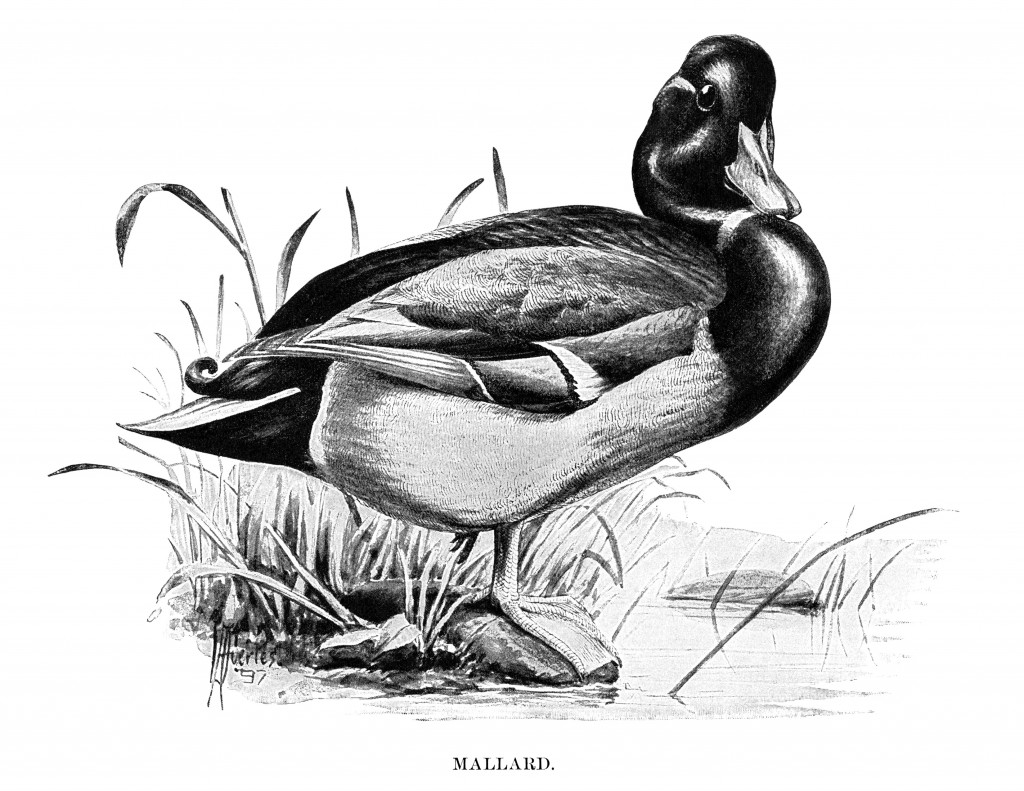
\includegraphics[width=\linewidth]{figures/duck}
  \caption{An illustration of a Mallard Duck. Picture from Mabel Osgood Wright, \textit{Birdcraft}, published 1897.}
  \label{fig:duck}
\end{figure}

\begin{table*}[t]
  \caption{A double column table.}
  \label{tab:commands}
  \begin{tabular}{ccl}
    \toprule
    A Wide Command Column & A Random Number & Comments\\
    \midrule
    \verb|\tabular| & 100& The content of a table \\
    \verb|\table|  & 300 & For floating tables within a single column\\
    \verb|\table*| & 400 & For wider floating tables that span two columns\\
    \bottomrule
  \end{tabular}
\end{table*}

\subsection{Tables}

Curabitur vitae nulla dapibus, ornare dolor in, efficitur enim. Cras fermentum facilisis elit vitae egestas. Mauris porta, neque non rutrum efficitur, odio odio faucibus tortor, vitae imperdiet metus quam vitae eros. Proin porta dictum accumsan \autoref{tab:commands}.

Duis cursus maximus facilisis. Integer euismod, purus et condimentum suscipit, augue turpis euismod libero, ac porttitor tellus neque eu enim. Nam vulputate est non tellus efficitur pharetra. Aenean molestie tristique venenatis. Nam congue pulvinar vehicula. Duis lacinia mollis purus, ac aliquet arcu dignissim ac \autoref{tab:freq}. 

\begin{table}[hb]% h asks to places the floating element [h]ere.
  \caption{Frequency of Special Characters}
  \label{tab:freq}
  \begin{tabular}{ccl}
    \toprule
    Non-English or Math & Frequency & Comments\\
    \midrule
    \O & 1 in 1000& For Swedish names\\
    $\pi$ & 1 in 5 & Common in math\\
    \$ & 4 in 5 & Used in business\\
    $\Psi^2_1$ & 1 in 40\,000 & Unexplained usage\\
  \bottomrule
\end{tabular}
\end{table}

Nulla sit amet enim tortor. Ut non felis lectus. Aenean quis felis faucibus, efficitur magna vitae. Curabitur ut mauris vel augue tempor suscipit eget eget lacus. Sed pulvinar lobortis dictum. Aliquam dapibus a velit.

\subsection{Listings and Styles}

Aenean malesuada fringilla felis, vel hendrerit enim feugiat et. Proin dictum ante nec tortor bibendum viverra. Curabitur non nibh ut mauris egestas ultrices consequat non odio.

\begin{itemize}
\item Duis lacinia mollis purus, ac aliquet arcu dignissim ac. Vivamus accumsan sollicitudin dui, sed porta sem consequat.
\item Curabitur ut mauris vel augue tempor suscipit eget eget lacus. Sed pulvinar lobortis dictum. Aliquam dapibus a velit.
\item Curabitur vitae nulla dapibus, ornare dolor in, efficitur enim.
\end{itemize}

Ut sagittis, massa nec rhoncus dignissim, urna ipsum vestibulum odio, ac dapibus massa lorem a dui. Nulla sit amet enim tortor. Ut non felis lectus. Aenean quis felis faucibus, efficitur magna vitae. 

\begin{enumerate}
\item Duis lacinia mollis purus, ac aliquet arcu dignissim ac. Vivamus accumsan sollicitudin dui, sed porta sem consequat.
\item Curabitur ut mauris vel augue tempor suscipit eget eget lacus. Sed pulvinar lobortis dictum. Aliquam dapibus a velit.
\item Curabitur vitae nulla dapibus, ornare dolor in, efficitur enim.
\end{enumerate}

Cras fermentum facilisis elit vitae egestas. Mauris porta, neque non rutrum efficitur, odio odio faucibus tortor, vitae imperdiet metus quam vitae eros. Proin porta dictum accumsan. Aliquam dapibus a velit. Curabitur vitae nulla dapibus, ornare dolor in, efficitur enim. Ut maximus mi id arcu ultricies feugiat. Phasellus facilisis purus ac ipsum varius bibendum.

\subsection{Math and Equations}

Curabitur vitae nulla dapibus, ornare dolor in, efficitur enim. Cras fermentum facilisis elit vitae egestas. Nam vulputate est non tellus efficitur pharetra. Vestibulum ligula est, varius in suscipit vel, porttitor id massa. Cras facilisis suscipit orci, ac tincidunt erat.
\begin{equation}
  \lim_{n\rightarrow \infty}x=0
\end{equation}

Sed pulvinar lobortis dictum. Aliquam dapibus a velit porttitor ultrices. Ut maximus mi id arcu ultricies feugiat. Phasellus facilisis purus ac ipsum varius bibendum. Aenean a quam at massa efficitur tincidunt facilisis sit amet felis. 
\begin{displaymath}
  \sum_{i=0}^{\infty} x + 1
\end{displaymath}

Suspendisse molestie ultricies tincidunt. Praesent metus ex, tempus quis gravida nec, consequat id arcu. Donec maximus fermentum nulla quis maximus.
\begin{equation}
  \sum_{i=0}^{\infty}x_i=\int_{0}^{\pi+2} f
\end{equation}

Curabitur vitae nulla dapibus, ornare dolor in, efficitur enim. Cras fermentum facilisis elit vitae egestas. Nam vulputate est non tellus efficitur pharetra. Vestibulum ligula est, varius in suscipit vel, porttitor id massa. Cras facilisis suscipit orci, ac tincidunt erat.

\section{Citations}

Some examples of references. A paginated journal article~\cite{Abril07}, an enumerated journal article~\cite{Cohen07}, a reference to an entire issue~\cite{JCohen96}, a monograph (whole book) ~\cite{Kosiur01}, a monograph/whole book in a series (see 2a in spec. document)~\cite{Harel79}, a divisible-book such as an anthology or compilation~\cite{Editor00} followed by the same example, however we only output the series if the volume number is given~\cite{Editor00a} (so Editor00a's series should NOT be present since it has no vol. no.), a chapter in a divisible book~\cite{Spector90}, a chapter in a divisible book in a series~\cite{Douglass98}, a multi-volume work as book~\cite{Knuth97}, an article in a proceedings (of a conference, symposium, workshop for example) (paginated proceedings article)~\cite{Andler79}, a proceedings article with all possible elements~\cite{Smith10}, an example of an enumerated proceedings article~\cite{VanGundy07}, an informally published work~\cite{Harel78}, a doctoral dissertation~\cite{Clarkson85}, a master's thesis~\cite{anisi03}, an finally two online documents or world wide web resources~\cite{Thornburg01, Ablamowicz07}.



%\clearpage

\bibliographystyle{ACM-Reference-Format}
\bibliography{ref}

\end{document}
\endinput
